\chapter{Results}

The three SLAM algorithms were evaluated regarding the computed trajectories, the resulting pointclouds and
the computational complexity. 

\section{Trajectory Evaluation}

	In order to evaluate the quality of the trajectory computed by the algorithms, the trajectory firstly had to be 
	transformed into the world reference of the ground truth data. This is because the algorithms usually initialize
	the origin with the first (key)frame and the groundtruth data doesn't. Furthermore, monocular visual slam algorithms 
	are generally not capable to extract the true scale. The alignment was performed using the method of Umeyama, described
	in the \ref{comp} section. 
	After alignment, as a first indicator for the accuracy of the computed trajectories, the trajectories were visually observed by 
	plotting the true position and the evaluated position into a coordiante system. The x, y and z axis were observed seperatly. This method 
    for comparing the trajectories is described in detail in section \ref{detail}. 	
	
	In figure \ref{fig:flight_path} the computed trajectories are plotted against the groundtruth for sequences MH01, V102 and V203 considering only the 
	x and y coordinate. These sequences 
	were selected, because they represent the results of the visual analalysis well. In the first sequence, MH01, all algorithms showed excellent results. 
	One reason for this could be, that in the first sequence, the camera only does very gentel movements, moving at an average speed of $0.41 ms^{-1}$. 
	
	The second image shows the sequence V102. Here
	
	% and here 

	\begin{figure}%
    \centering
    \subfloat[\centering MH01]{{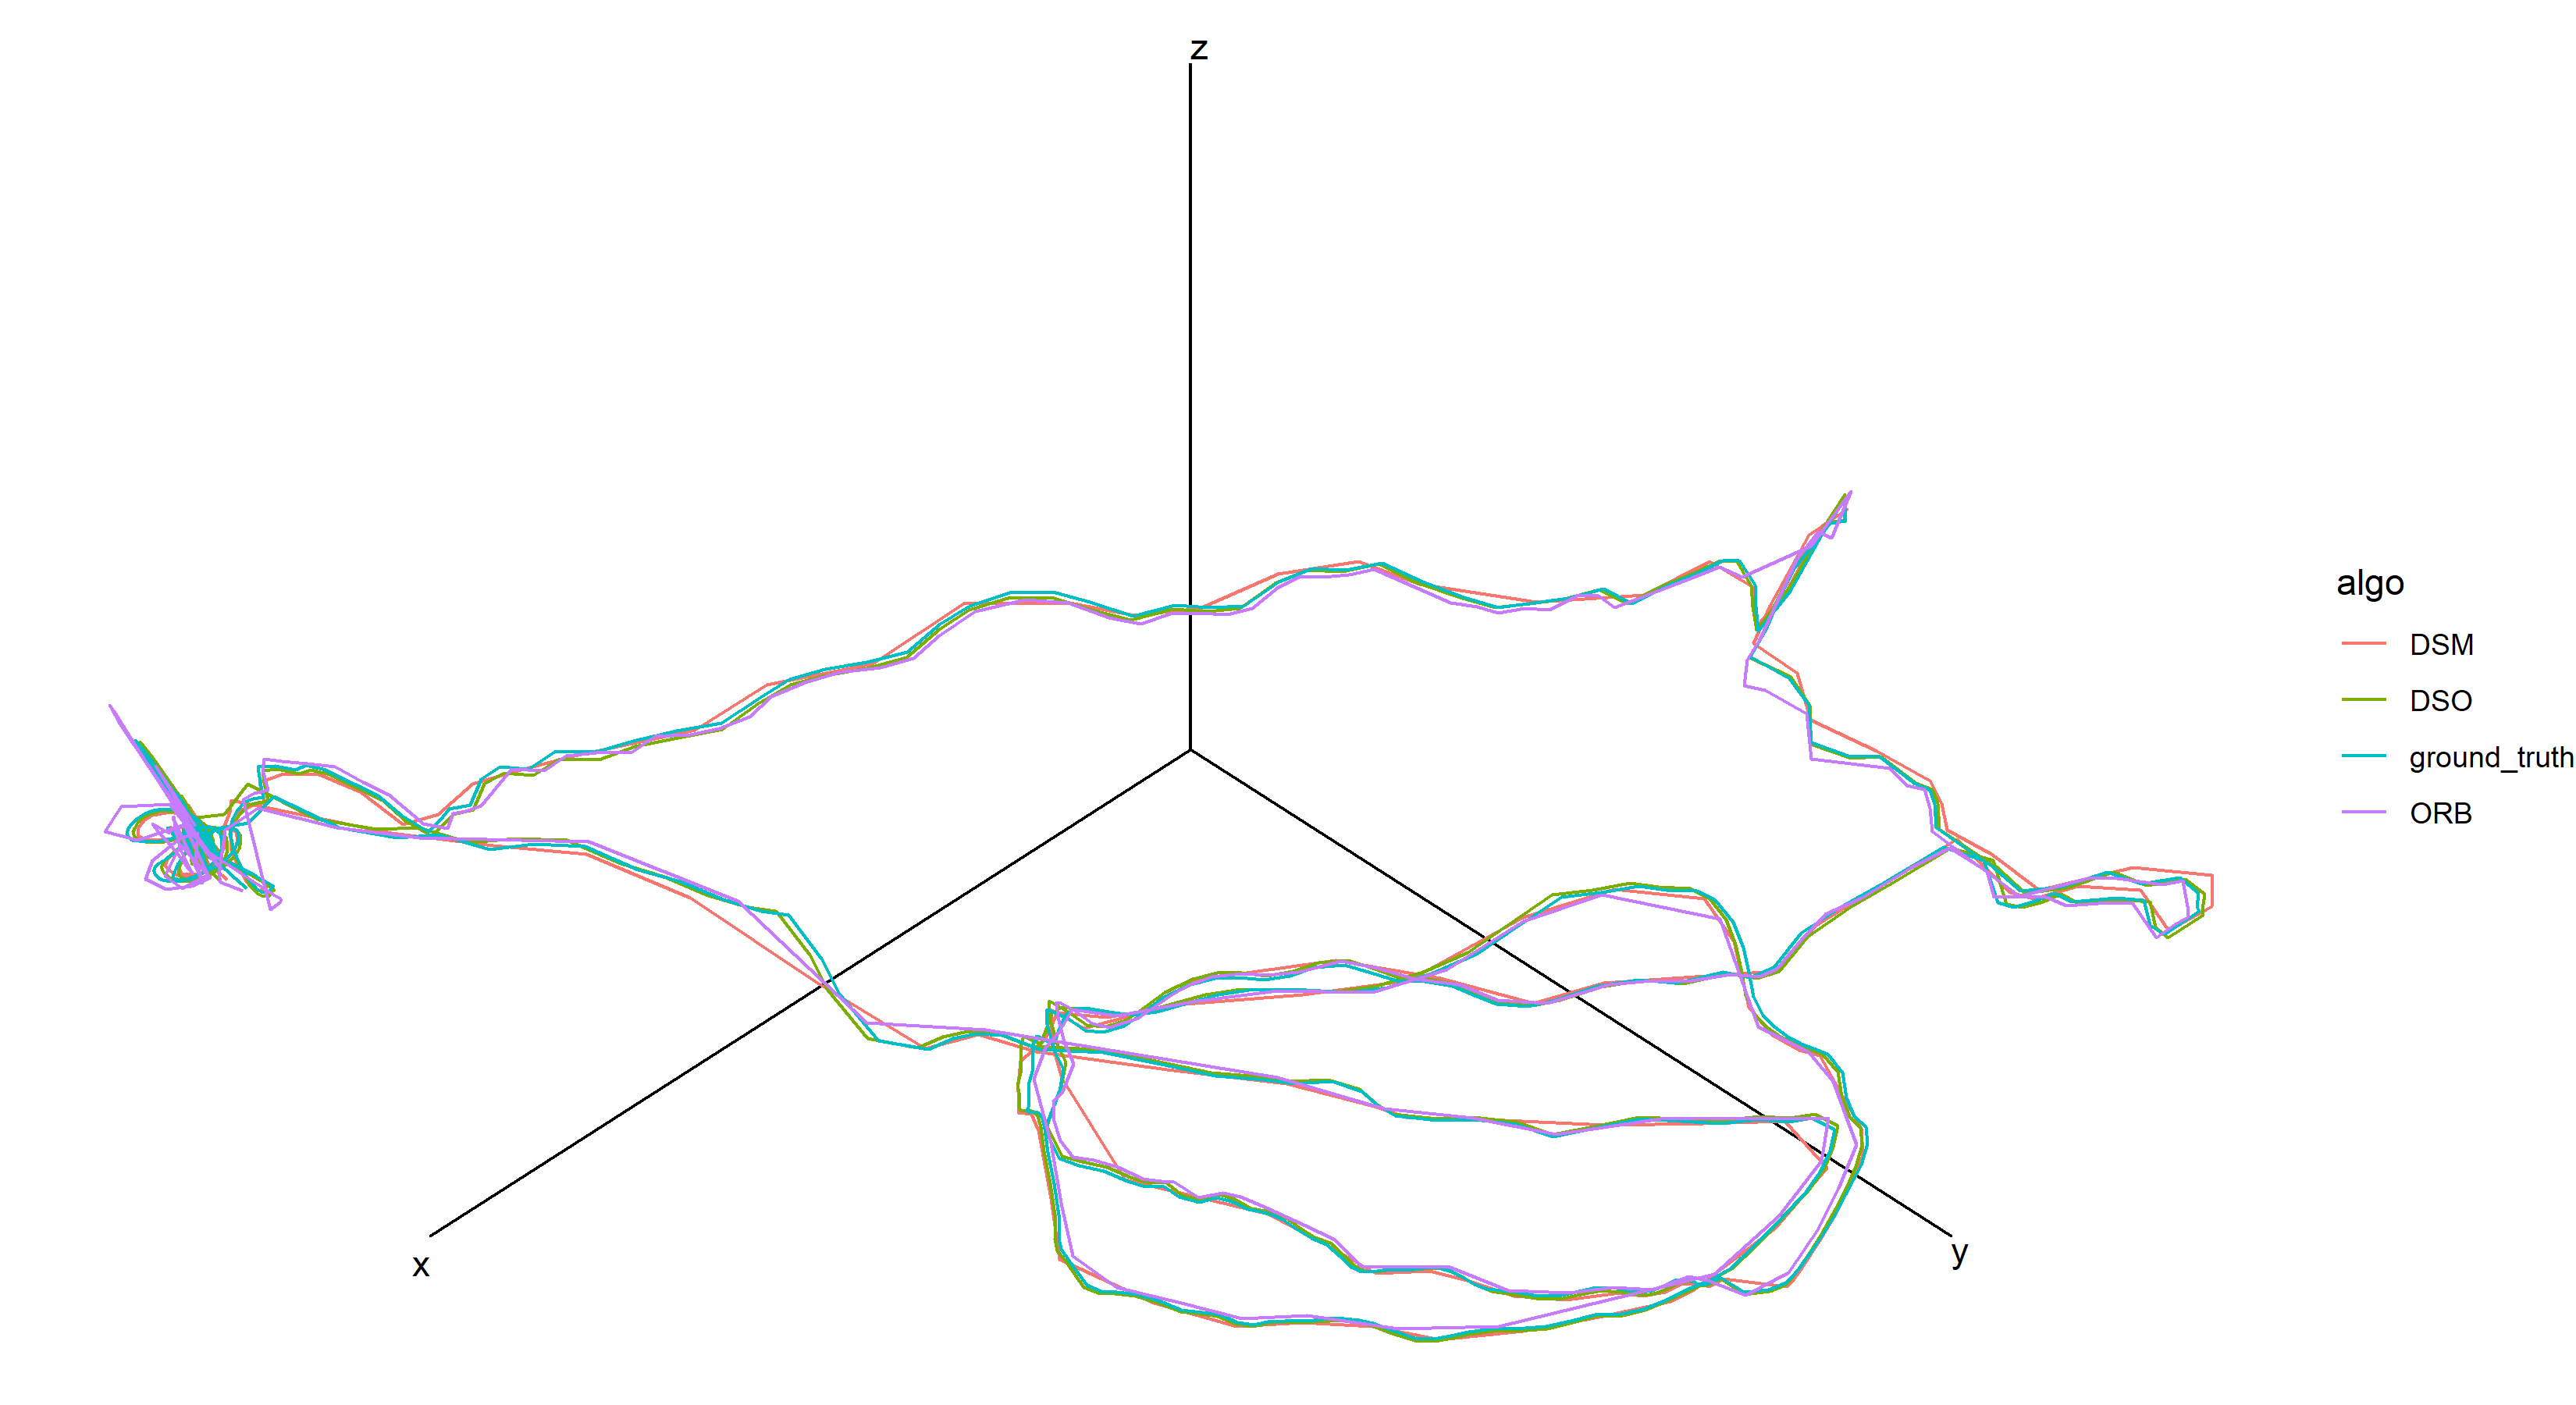
\includegraphics[width=9cm]{img/traj_perf.png} }}%
    \qquad
    \subfloat[\centering V102]{{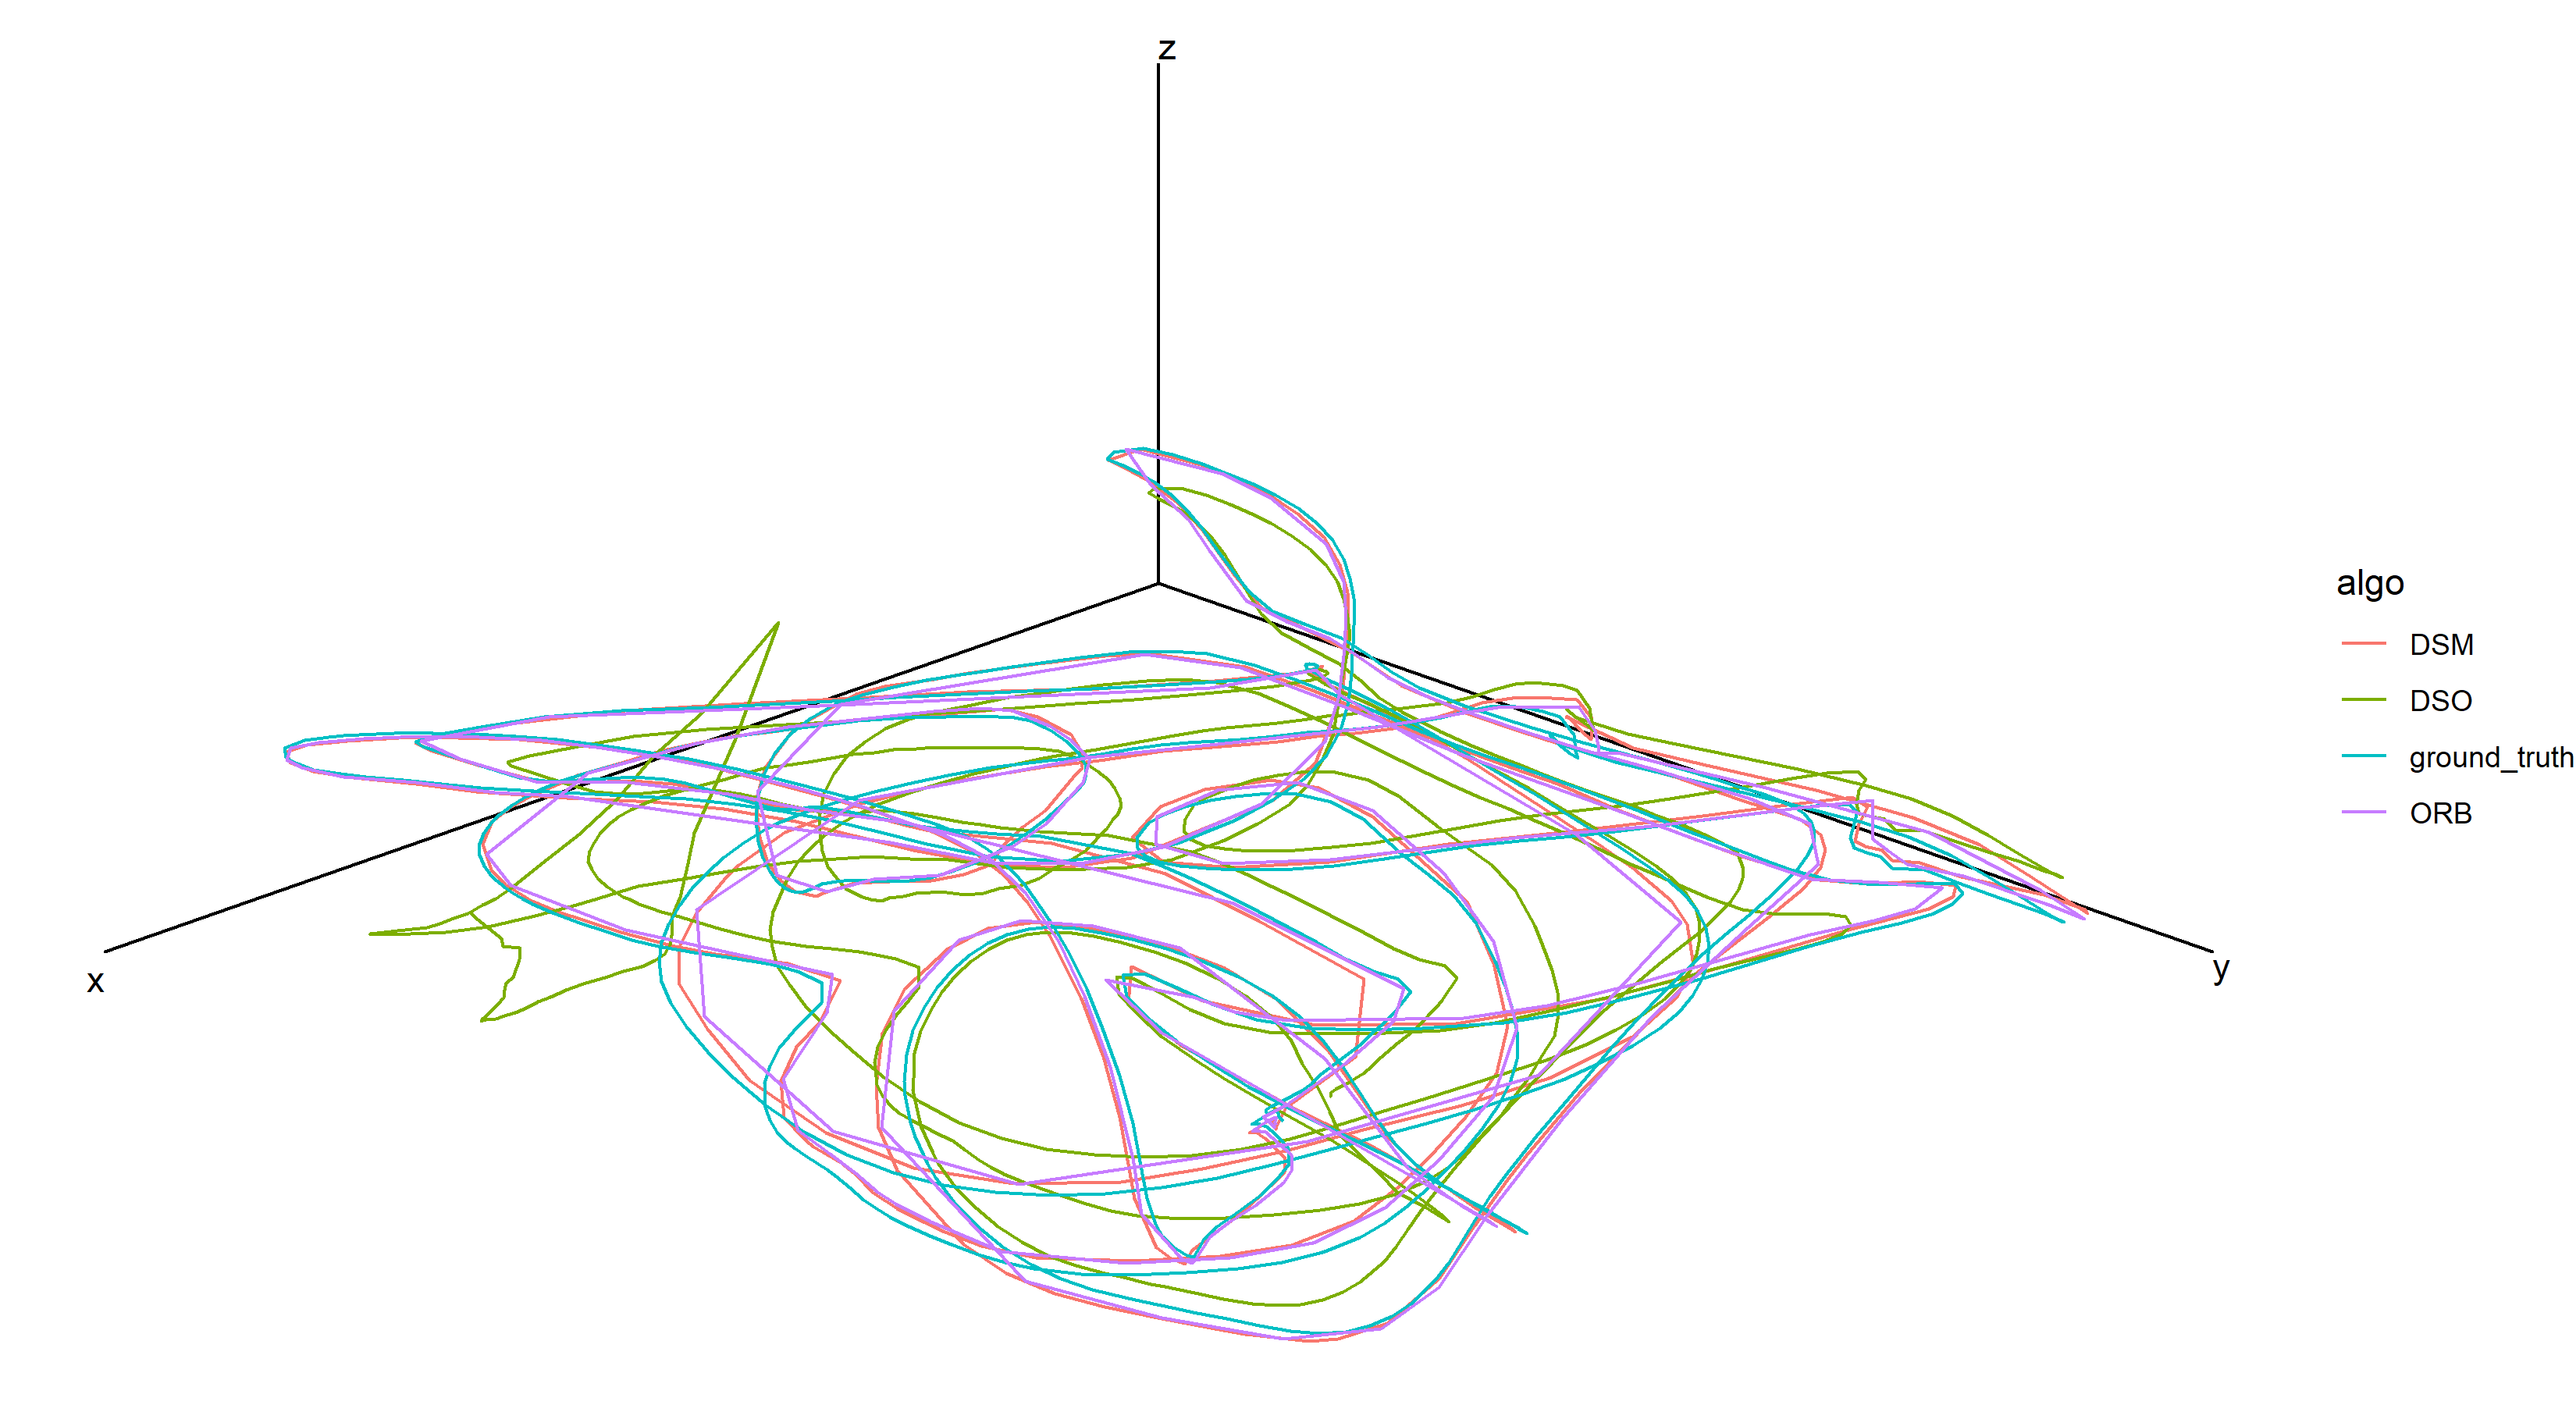
\includegraphics[width=9cm]{img/traj_dso.png} }}%
	\qquad
    \subfloat[\centering V203]{{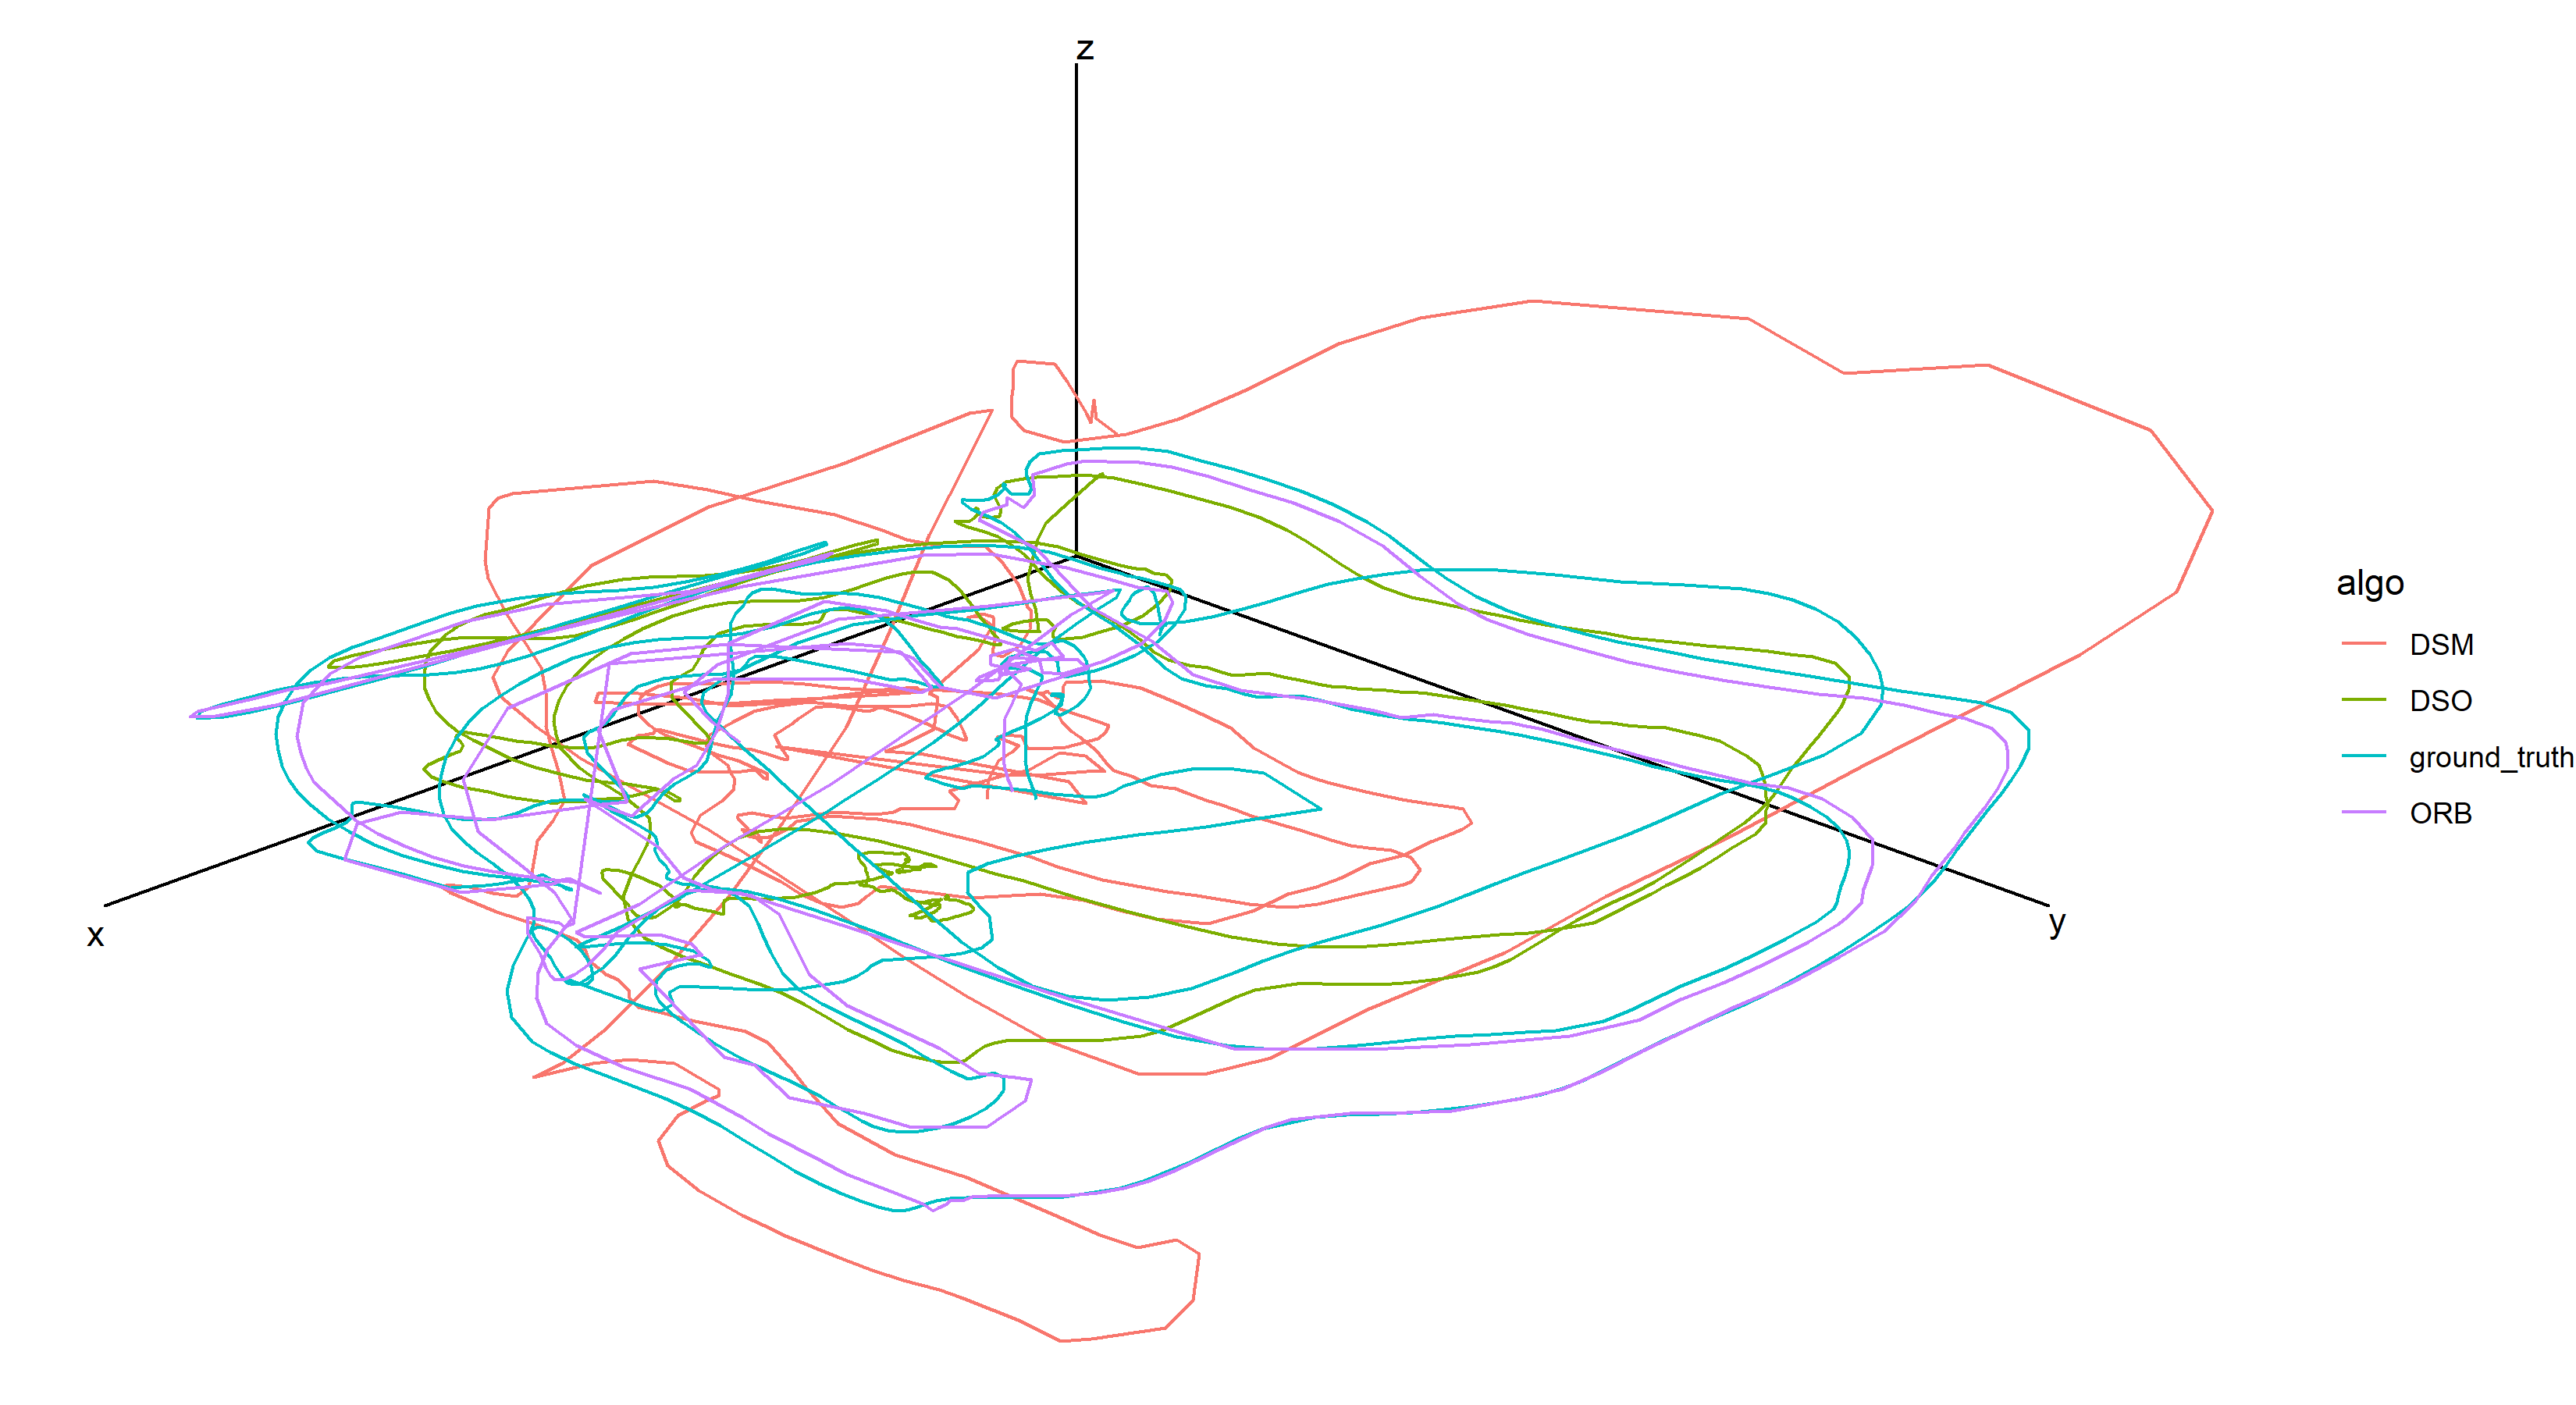
\includegraphics[width=9cm]{img/traj_last.png} }}%
    \caption{
	Ground truth flight path and evaluated flight path of each algorithm after alignment with the method of Umeyama in the x and y axis in meters. 
	Left the sequence MH01, middle the sequence V102 and right the sequence V203 is displyed.
	}%
    \label{fig:flight_path}%
	\end{figure}
	
	
	Furthermore, the eucleadian distances between position of the keyframe and the true postion of the latter are computed. For a keyframe, 
	the entry of the groundtruth data with the lowest distance in time to the time the keyframe was inserted is taken as reference point. 
	This is justifiable, since the true position is sampled at a frequency of over 200 points per second. 
	
	In figure \ref{fig:boxplot_traj} a boxplot of all computed distances over all sequences is displayed. 
	
	% result here. 
	
	
	\fig{img/boxplot_dist.png}{Boxplot of all euclideans distances between the ground truth position of the keyframe and 
	the evaluated position after alignment with the method of Umeyama. Outliers greater than 1.5 are not displayed.
	}{fig:boxplot_traj}{0.8}
	
	
	\fig{img/pos_error.png}{The positional error over time in meters. The vertical lines indicate the beginning of a new sequence}{fig:pos_error}{1}
	


\section{Pointcloud Evaluation}

For the evaluation of the computed point clouds, these point clouds were first visually observed, as described in section \ref{sec}. 
Figure \ref{fig:pointcloud} shows the evaluated point clouds aligned with the ground truth point cloud for sequence V101. This is a sequence, 
where the tracking of the trajectory was successfull for all three algorithms, thus, the errors of the resulting point clouds can not 
be a result of errors in alignment. 

What becomes clear at first glance is, that as mentioned, ORB generates only few points, since only found keypoints are mapped in feature based methods.
 To give these  points better visibilty, the point size was doubled in the ORB image. DSM and DSO slam generate point clouds with significant higher 
 density, where all structures of the room are clearly visible at first glance. 
 
 However, the advantace of ORB-SLAM over the other two direct methods 
 is the recognizing of clear features in terms of strucural differences in the scenes. Though, DSO and DSM also regard the differences in pixel intensities
 ORB, as described in section \ref{refasdf}, detects the features on different scale levels and ensures, that the regarded features are in fact significant. 
 This also became clear when observing the point cloud. All significant features, and therefore important features for autonomous navigation, were successfully 
 marked with a computed point. For example, this can be seen at the leiter?? in image three of figure \ref{fig:pointcloud}, where all sprossen contain at least 
 on point. 

 
 After closely observing the point clouds, it became clear, that the point clouds of DSO, often times generate point clouds, where multiple layers of 
 points were falsly generated, where all points had the same clear distance to the ground truth point cloud. This may be a result of working of DSO slam, 
 where keyframes, that are marginalized, are removed permanently. When revisiting areas, the points are again generated. This means that all errors made
 in the sequence accumulate and when an area is revisited, significant errors in the point cloud can be made. This can be seen when looking at the 
 third image closely. When looking at the matraccess in the middle of the room, the accumulated error expresses itself by points hovering in the air 
 in a clear plane. 
 
 

	\begin{figure}%
    \centering
    \subfloat[\centering ORB]{{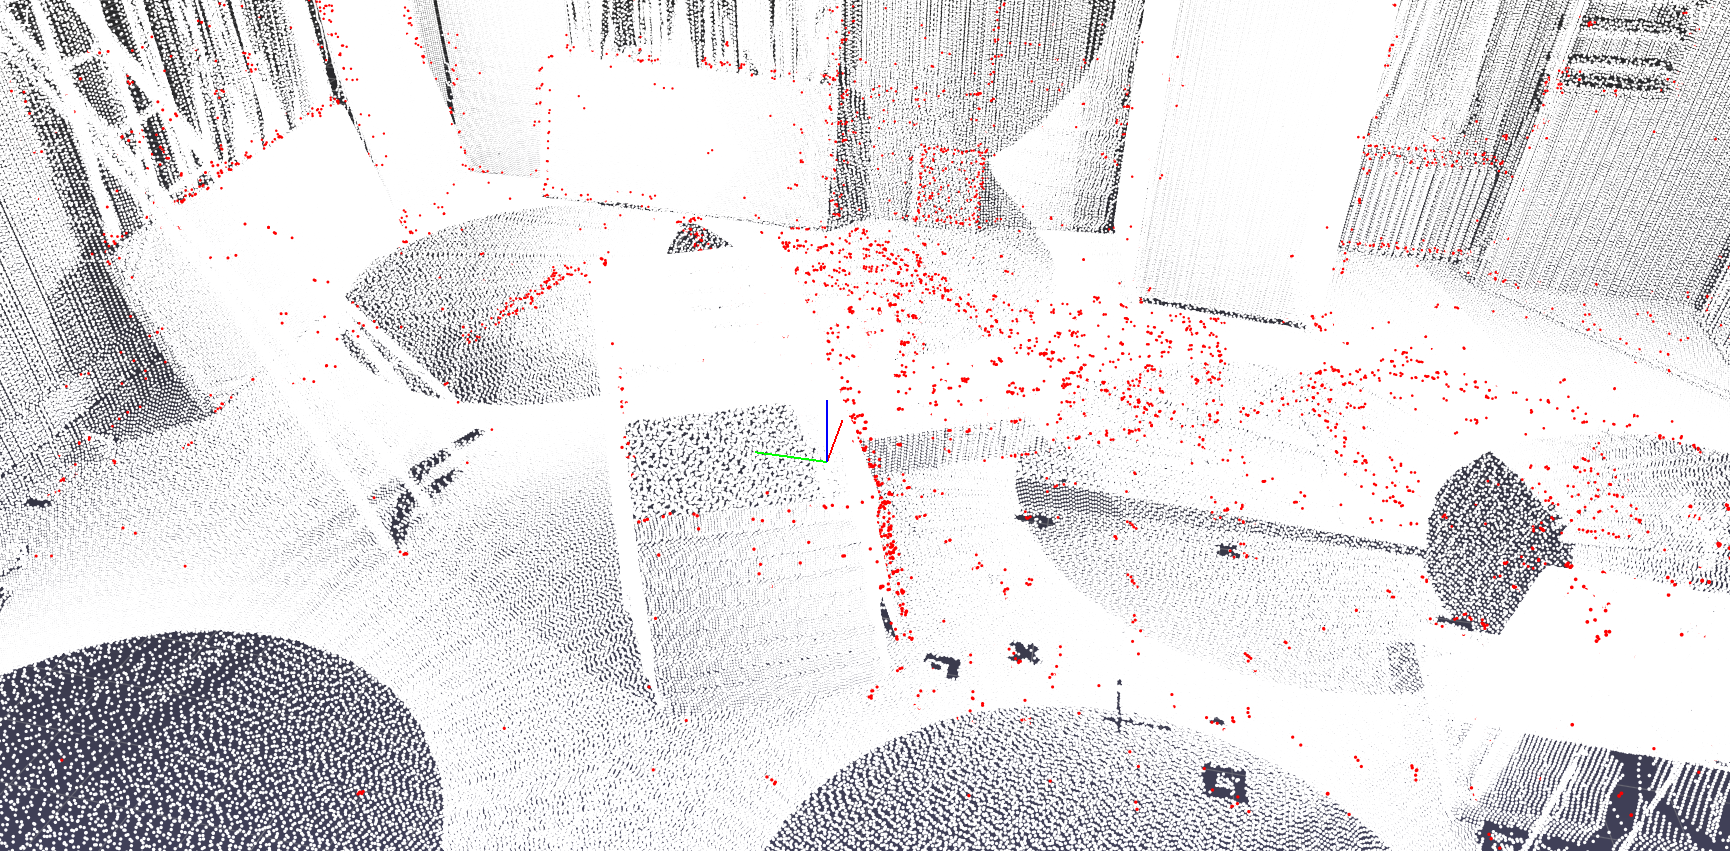
\includegraphics[width=5cm]{img/pointcloud_orb} }}%
    \qquad
    \subfloat[\centering DSM]{{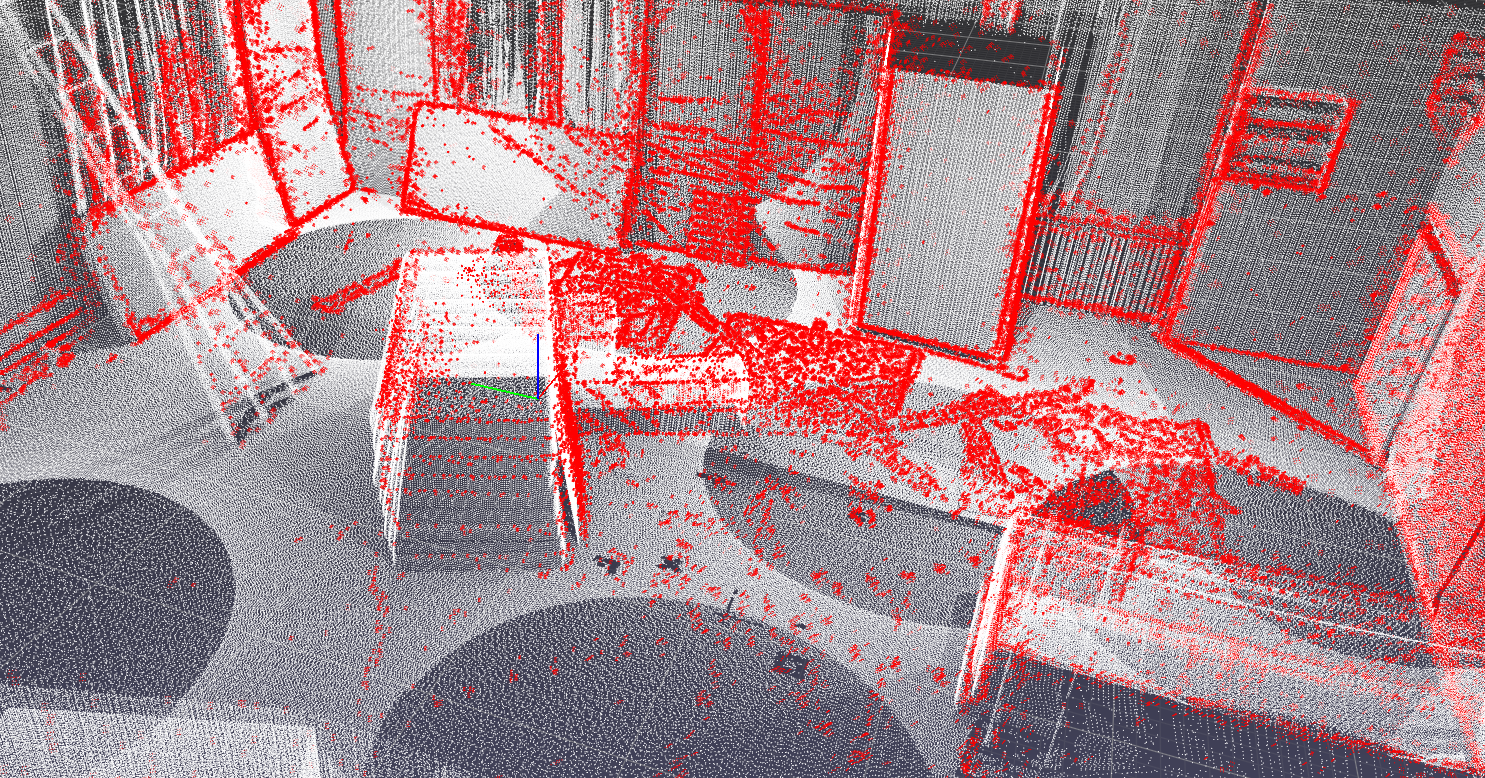
\includegraphics[width=5cm]{img/pointcloud_dsm} }}%
	\qquad
    \subfloat[\centering DSO]{{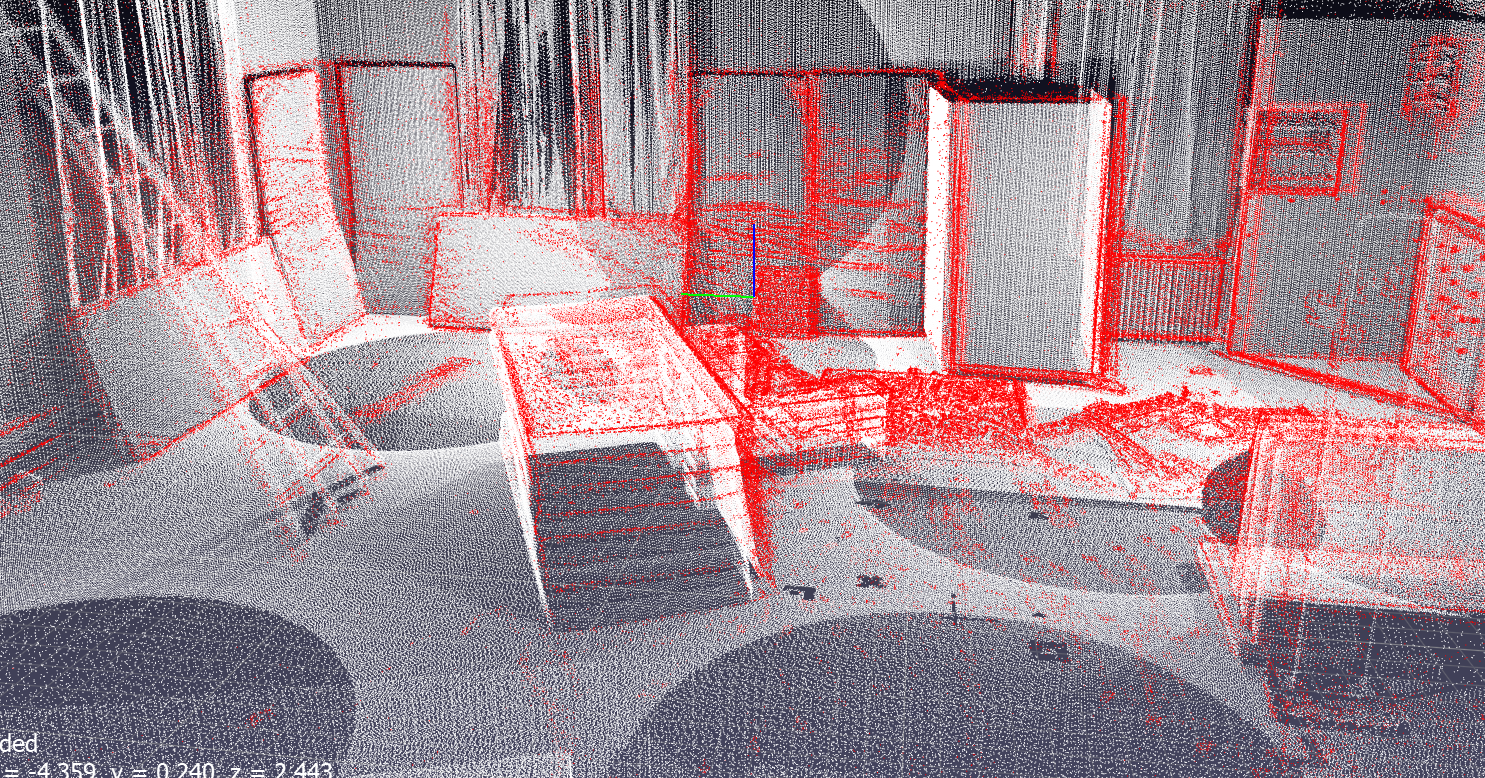
\includegraphics[width=5cm]{img/pointcloud_dso} }}%
    \caption{The groundtruth of the Pointcloud from Sequence V101 (white points) and the evaluated points by each algorithm (red points). 
	The points in Figure (a) are wtice as large for better visability (ORB-SLAM generates only few points). 
	}%
    \label{fig:pointcloud}%
	\end{figure}
	
	
	The density can also be expressed by numbers. The significant difference of the numbers of points can be seen in table \ref{table:pointcloud}. While 
	ORB slam only generates close to 10000 points in the sequences DSM slam generates more than 500000 points in most sequences and DSO more than 200000 
	in most sequences. 
	
	\begin{table}
	\caption{Number and accuracy of evaluated points of each algorithm}
	\begin{tabular}{ |p{3cm}||p{3cm}|p{3cm}|p{3cm}|  }
	\hline
	Sequence Name& ORB & DSM & DSO \\
	\hline
	MH\_01\_easy & 8958 (/) & 675720 (/) & 361633 (/)\\
	MH\_02\_easy & 8692 (/) & 700920 (/) & 343804 (/)\\
	MH\_03\_medium & / (/) & 614264 (/) & 371752 (/)\\
	MH\_04\_difficult & 7943 (/) & 495752 (/) & 208445 (/)\\
	MH\_05\_difficult & 8373 (/) & 517712 (/) & 232415 (/)\\
	V1\_01\_easy & 7075 (0.049) & 6108440 (0.066) & 374257 (0.066)\\
	V1\_02\_medium & 6517 (0.042) & 648440 (0.187) & 366513 (1.458)\\
	V1\_03\_difficult & / (/) & 775080 (0.092) & 448212 (0.459)\\
	V2\_01\_easy & / (/) & 584552 (0.58) & 247905 (0.086)\\
	V2\_02\_medium & / (/)& 733992 (0.078) & 490608 (0.104)\\
	V2\_03\_difficult & / (/) & 921312 (0.645) & 465396 (0.677)\\
	\hline
	\end{tabular}
	\label{table:pointcloud}
	\end{table}
	
	
	\fig{img/pq_dist.png}{Boxplot of the eucleadian distances between an evaluated point and the closest point of the ground truth point cloud.
	For computational feasibility, for each sequence and algorithm, 500 points for evaluation are sampled randomly}{fig:boxplot_pq}{0.8}
	
	

\section{Calculation Time}

	\begin{table}
	\caption{Computation Time (excluded time needed for initialization) of each Sequence and Algorithm}
	\begin{tabular}{ |p{3cm}||p{3cm}|p{3cm}|p{3cm}|  }
	\hline
	Sequence Name& Computation Time in $s$ ORB & Computation Time in $s$ DSM & Computation Time in $s$ DSO \\
	\hline
	MH\_01\_easy & 257 & 1098 & 749\\
	MH\_02\_easy & 209 & 984 & 690\\
	MH\_03\_medium & 198 & 1369 & 707\\
	MH\_04\_difficult & 165 & 896 & 504\\
	MH\_05\_difficult & 193 & 825 & 633\\
	V1\_01\_easy & 253 & 1383 & 905\\
	V1\_02\_medium & 150 & 1550 & 820\\
	V1\_03\_difficult & 186 & 2262 & 1134\\
	V2\_01\_easy & 187 & 1045 & 612\\
	V2\_02\_medium & 162 & 1675 & 1522\\
	V2\_03\_difficult & 143 & 1600 & 793\\
	\hline
	\end{tabular}
	\label{table:comp_time}
	\end{table}

